\documentclass{article} % For LaTeX2e
\usepackage{nips_adapted,times}
\usepackage{hyperref}
\usepackage{url}

\usepackage{pdfpages} 
\title{Our Awesome ML Project}


\author{
Author 1 \\
Roll No. \\
\And
Author 1 \\
Roll No. \\
\AND
Author 1 \\
Roll No. \\
\And
Author 1 \\
Roll No. \\
\And
Author 1 \\
Roll No. \\
}

% The \author macro works with any number of authors. There are two commands
% used to separate the names and addresses of multiple authors: \And and \AND.
%
% Using \And between authors leaves it to \LaTeX{} to determine where to break
% the lines. Using \AND forces a linebreak at that point. So, if \LaTeX{}
% puts 3 of 4 authors names on the first line, and the last on the second
% line, try using \AND instead of \And before the third author name.

\newcommand{\fix}{\marginpar{FIX}}
\newcommand{\new}{\marginpar{NEW}}

\nipsfinalcopy

\begin{document}

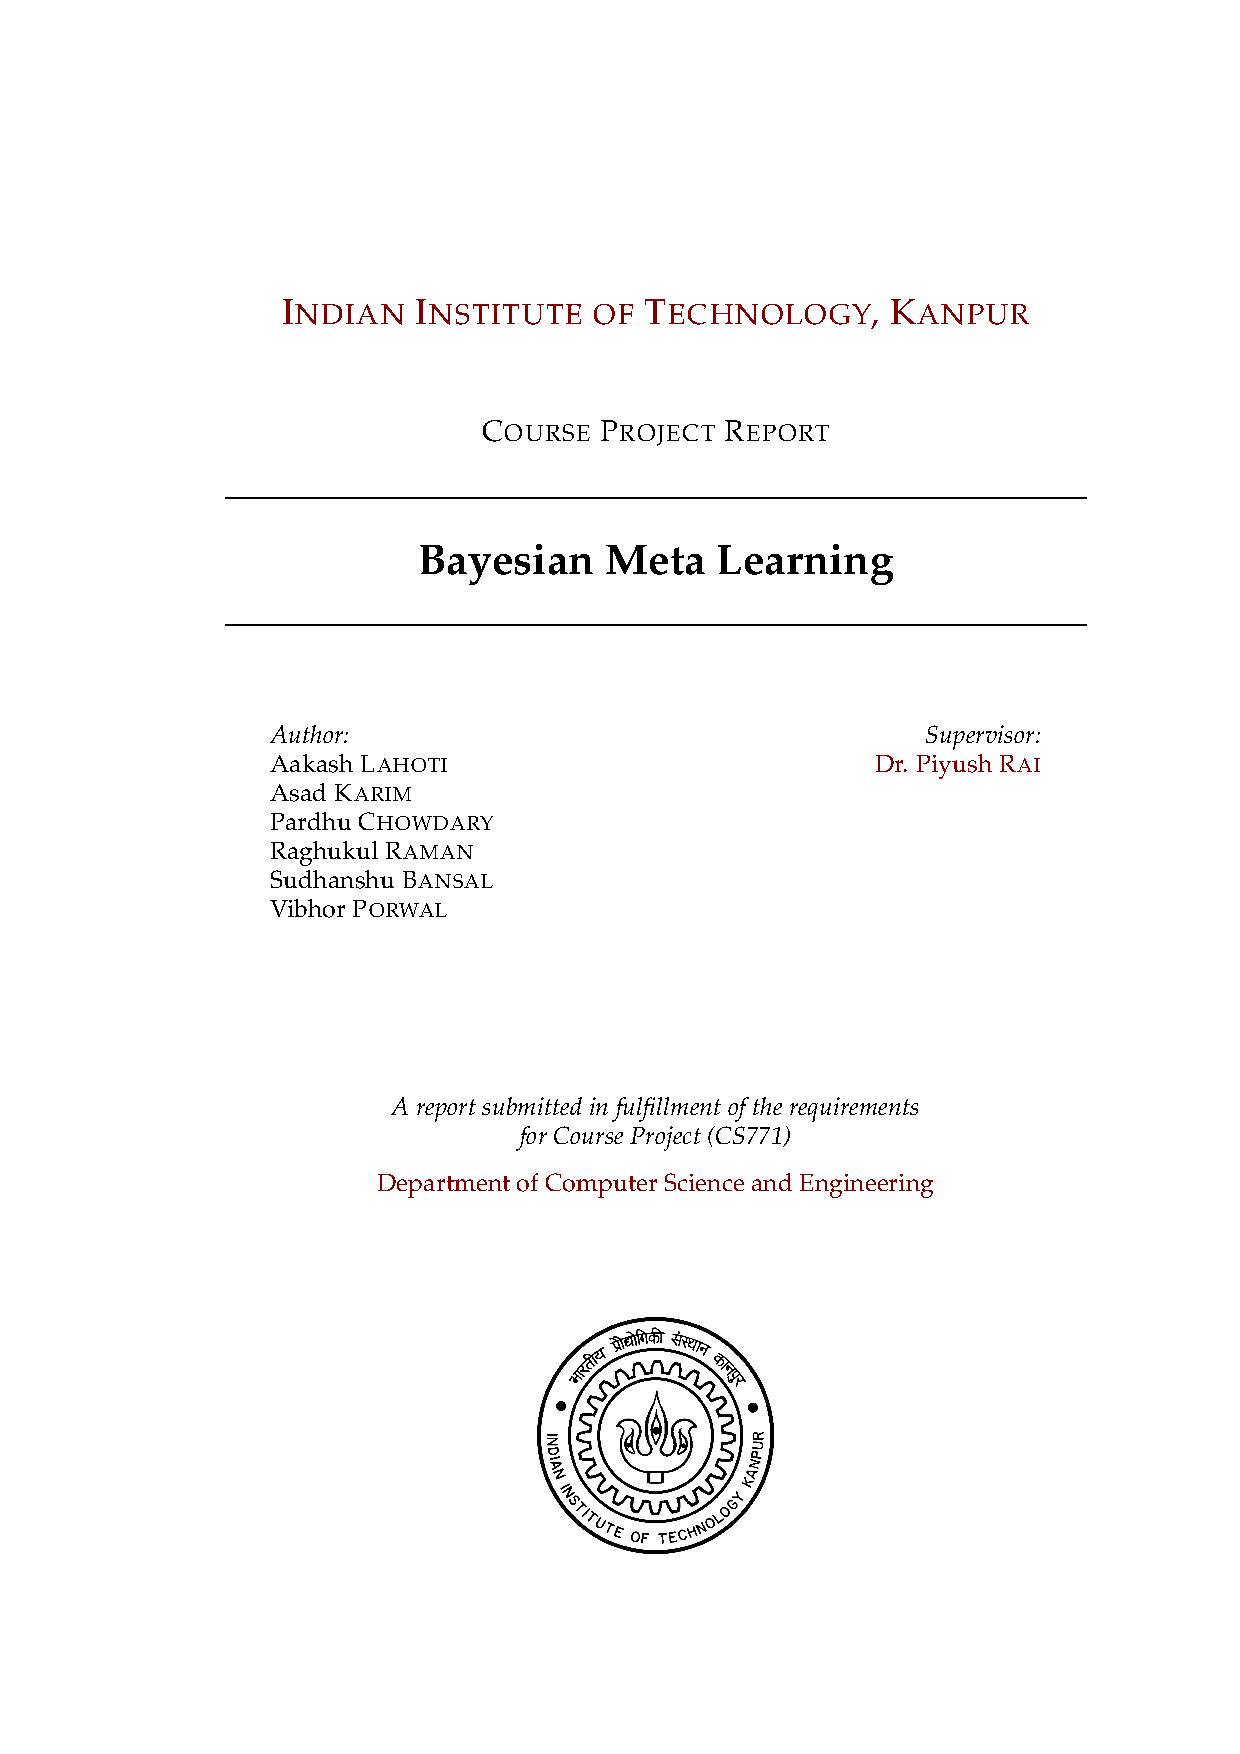
\includepdf[page={1}]{first_page.pdf}


\section{Abstract}

Our project is on..

\subsection{Subsection (if any) Name}

....

\section{Literature Review}

....

\subsection{Algorithm Review}

....

\subsection{Bayesian ML}

....

\subsection{Reinforcement Learning}

....

\section{Experiments}

....

\subsection{Regression}

....

\subsection{Classification}

....

\section{Conclusion}

....

\subsection{Subsection (if any) Name}

....

\section{Future Work}

....

\subsection{Subsection (if any) Name}

....

\subsubsection*{Acknowledgments}

....

\subsubsection*{References}
% may use bixtex to automatically generate the list of references or
% enter these manually below

\small{
[1] Chelsea Finn, Pieter Abbeel and Sergey Levine\\
\textit{Model-Agnostic Meta-Learning for Fast Adaptation of Deep Networks}

[2] Taesup Kim
, Jaesik Yoon
, Ousmane Dia1
, Sungwoong Kim
,
Yoshua Bengio
and Sungjin Ahn\\
\textit{Bayesian Model-Agnostic Meta-Learning}

[3] Erin Grant, Chelsea Finn, Sergey Levine, Trevor Darrell, Thomas Griffiths\\
\textit{Recasting Gradient-based Meta-Learning as
hierarchical Bayes}
}

\end{document}
